\section{Additional results for the one-variance baseline}\label{app:baseline}
\subsection{What happens to the meeting-risk ranges?}
For dates that fit a stated tolerance, we solve the endpoint problems \eqref{eq:LP}. Figure~\ref{fig:empiricalranges} uses 18 June, the earliest sample date on which all three background specifications fit at 1 bp. Selecting it by this rule makes the example reproducible; it is not presented as a typical date.

For the 16 September meeting, constant background gives a range of $[689,1149]$ bp$^2$. With 90-day cells it is $[507,1407]$; with a separate rate in each expiry gap it is $[0,1450]$. For the 27 January 2027 meeting, the constant-background range is $[1870,2990]$ bp$^2$, whereas both flexible specifications permit zero. Thus a claim of strictly positive meeting risk can depend on the background restriction even when all specifications fit within the same price tolerance. For scale, the constant-background September range corresponds to a meeting standard deviation of approximately 26.2--33.9 bp; the expiry-gap range allows 0--38.1 bp.

The zero lower bounds with an expiry-gap background are structural: replacing each gap's event contribution by an equal amount of background variance leaves its observed increment unchanged. The data illustrate the size of the compatible ranges, not a newly discovered source of nonidentification.

The total variance of all eight meetings in this example is constrained to $[5308,6582]$ bp$^2$ under constant background, $[507,8892]$ with 90-day cells, and $[0,9376]$ with an expiry-gap background. Grouping meetings does not remove uncertainty about how much risk belongs to meetings at all. These are sharp conditional ranges for the diagnostic's interval observations; different coordinate endpoints need not occur at the same allocation.

\begin{figure}[ht]
\centering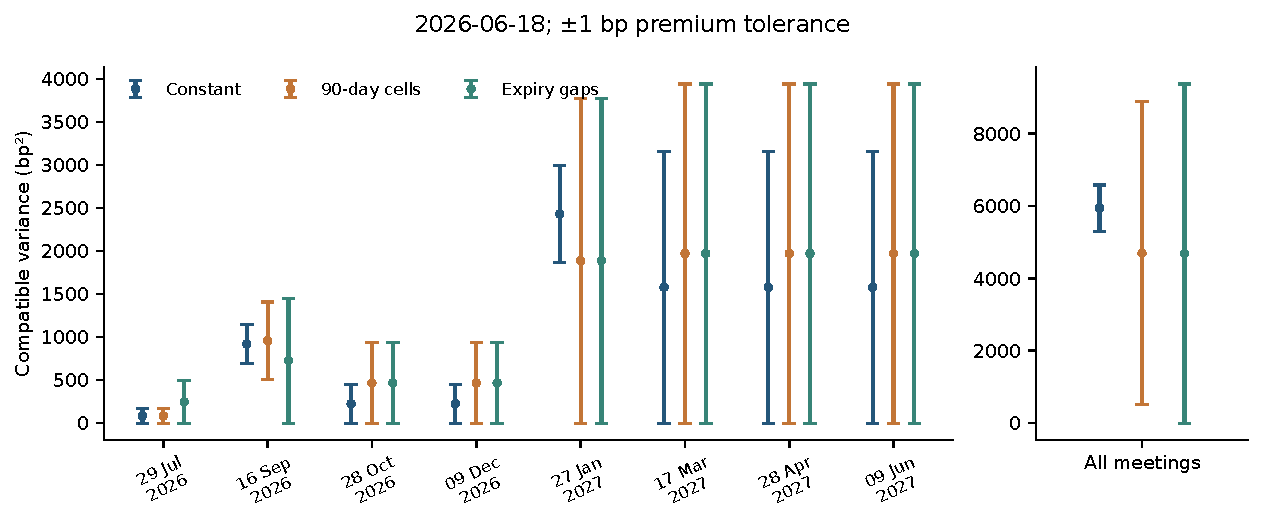
\includegraphics[width=\textwidth]{figures/empirical_ranges.pdf}
\caption{Compatible meeting variances in the normal diagnostic on 18 June 2026, using every selected strike within a 1 bp premium tolerance. Left: marginal ranges by meeting. Right: the jointly optimized total across meetings, on a separate vertical scale. All endpoints are shown without clipping; the individual and total panels have different scales. The markers are interval midpoints, not point estimates.}\label{fig:empiricalranges}
\end{figure}

\FloatBarrier
\subsection{Omitted-strike and omitted-expiry checks}
Figure~\ref{fig:empiricalchecks} collects the omitted-strike and same-expiry midcurve diagnostics. Two exercises check information outside a fitted input. First fit \eqref{eq:normalproxy} exactly to the closest out-of-the-money strike in each standard chain and price its other selected strikes. Across 555 chains, the median largest omitted-strike error is 1.000 bp and the maximum is 3.851 bp. Allowing the variance to fit all strikes helps: the median best possible uniform error within one chain is 0.747 bp. It still exceeds the tighter tolerance scenarios.

The second exercise withholds the entire second chronological expiry on each date. All remaining selected strikes constrain the constant-background model. The parameters and observation matrix retain the full meeting horizon, so removing the expiry does not silently remove an event parameter. At 0.5 bp, the training set is feasible on four dates; at 1 bp, on 26. On those dates, optimize the variance at the omitted expiry over all feasible allocations and convert its extrema to a premium range at the held-out chain's closest strike. Every held quote interval overlaps its prediction range. The median prediction width is 1.390 bp at the tighter tolerance and 3.253 bp at the wider one. This fixed screen produces no out-of-range candidate. The other dates fail at the training stage and supply no calibrated prediction interval.

This is a same-date omitted-contract check, not a forecast on a later date. It tests only the closest strike of the withheld chain; overlap there does not establish a fit to that chain's other strikes. The small feasible sample and the width of the ranges also prevent interpreting the absence of a candidate as evidence that the model is accurate or that the market offers no relative-value opportunities.


\begin{figure}[ht]
\centering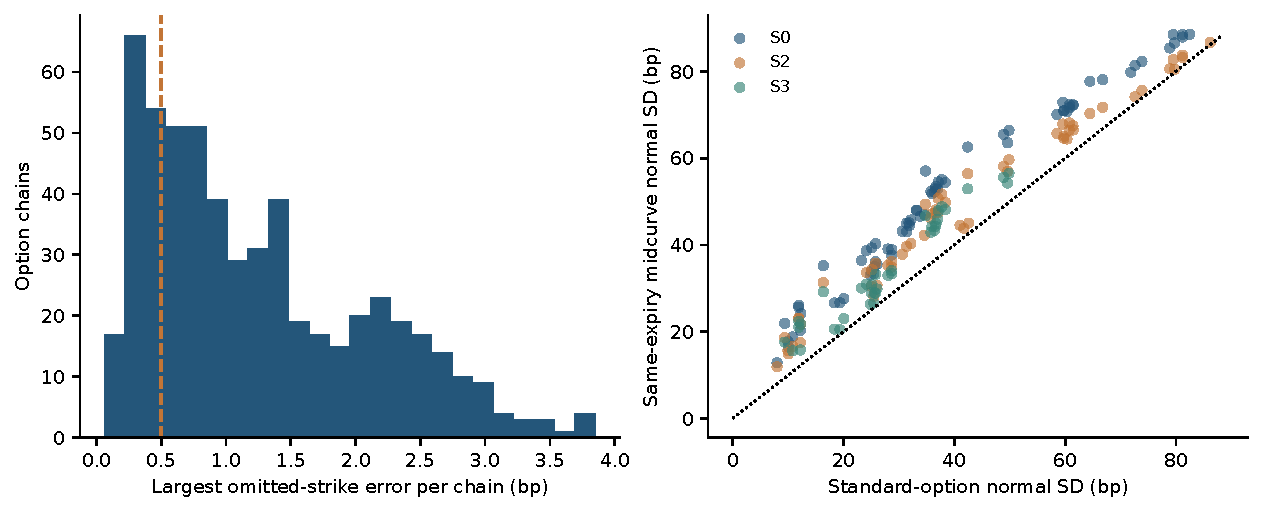
\includegraphics[width=\textwidth]{figures/empirical_price_checks.pdf}
\caption{Checks beyond a closest-strike fit. Left: largest error at omitted strikes in each standard chain; the dashed line is 0.5 bp. Right: normal standard deviations inferred separately from closest strikes in standard options and same-expiry midcurves. Equality is the parallel diagnostic's prediction. Differences can reflect maturity loadings, distributional shape, or exercise effects; this experiment does not identify their separate contributions.}\label{fig:empiricalchecks}
\end{figure}

\FloatBarrier
